\documentclass[14pt,a4paper]{article}

\usepackage{textgreek}
\usepackage[utf8x]{inputenc}
\usepackage{graphicx}
\usepackage[export]{adjustbox}
\usepackage[a4paper, portrait, margin=1in]{geometry}
\usepackage[ukrainian]{babel}
\usepackage{cmap}
\usepackage{etoolbox}
\usepackage{caption}
\usepackage{booktabs}
\usepackage{listings}
\usepackage{pgfplots}
\usepackage{xcolor} 
\usepackage{titlesec}
\usepackage{setspace}
\usepackage{fancyhdr} 
\usepackage{amsmath} 
\usepackage{amsthm}
\usepackage{hyperref}
\usepackage{amsmath} 
\usepackage{bm} 
\usepackage[square,sort,comma,numbers,super]{natbib}
\usepackage{caption}
\usepackage{float}

\graphicspath{ {./Images/} }

\title{\Huge \textbf{Інструкція до інсталяції та конфігурування системи AtOM. Access to Memory} }
\date{}

\lstset{
    language=bash,
    frame=single,             % додає рамку навколо коду
    backgroundcolor=\color{lightgray}, % встановлює сірий фон
    numbers=left,             % додає нумерацію рядків ліворуч
    numberstyle=\tiny\color{black}, % налаштовує стиль нумерації рядків
    basicstyle=\ttfamily\small, % встановлює стиль шрифту
    keywordstyle=\color{blue}, % колір для ключових слів
    breaklines=true,          % переносить рядки, якщо вони довгі
    columns=fullflexible
}

\begin{document}

\begin{titlepage}
    \pagecolor{green} 
    \color{black}
    \maketitle
    \thispagestyle{empty}
    
	\begin{center}
	
\includegraphics[max width=1.5\textwidth]{Images/logo_grn.png}
	\end{center}    
    
    \vspace*{8cm}
    \center \textbf{Львівський національний університет імені Івана Франка}
    \center \textbf{Львів 2024}

\end{titlepage}

\pagecolor{white}
\color{black}

\newpage

\pagenumbering{Roman}
\tableofcontents
\newpage
\pagenumbering{arabic}

\section{Загальна інформація}
\begin{large}
\textbf{AtoM} визначається як \textbf{"Access to Memory"}. Це є веб-програма з відкритим вихідним для архівного опису та доступу на основі стандартів у багатомовному середовищі з \textbf{мультирепозитарною системою}, тобто такою, яка використовується мережею архівних установ або інших типів сховищ.

\subsection{Технічний огляд}
    
	\begin{center}
	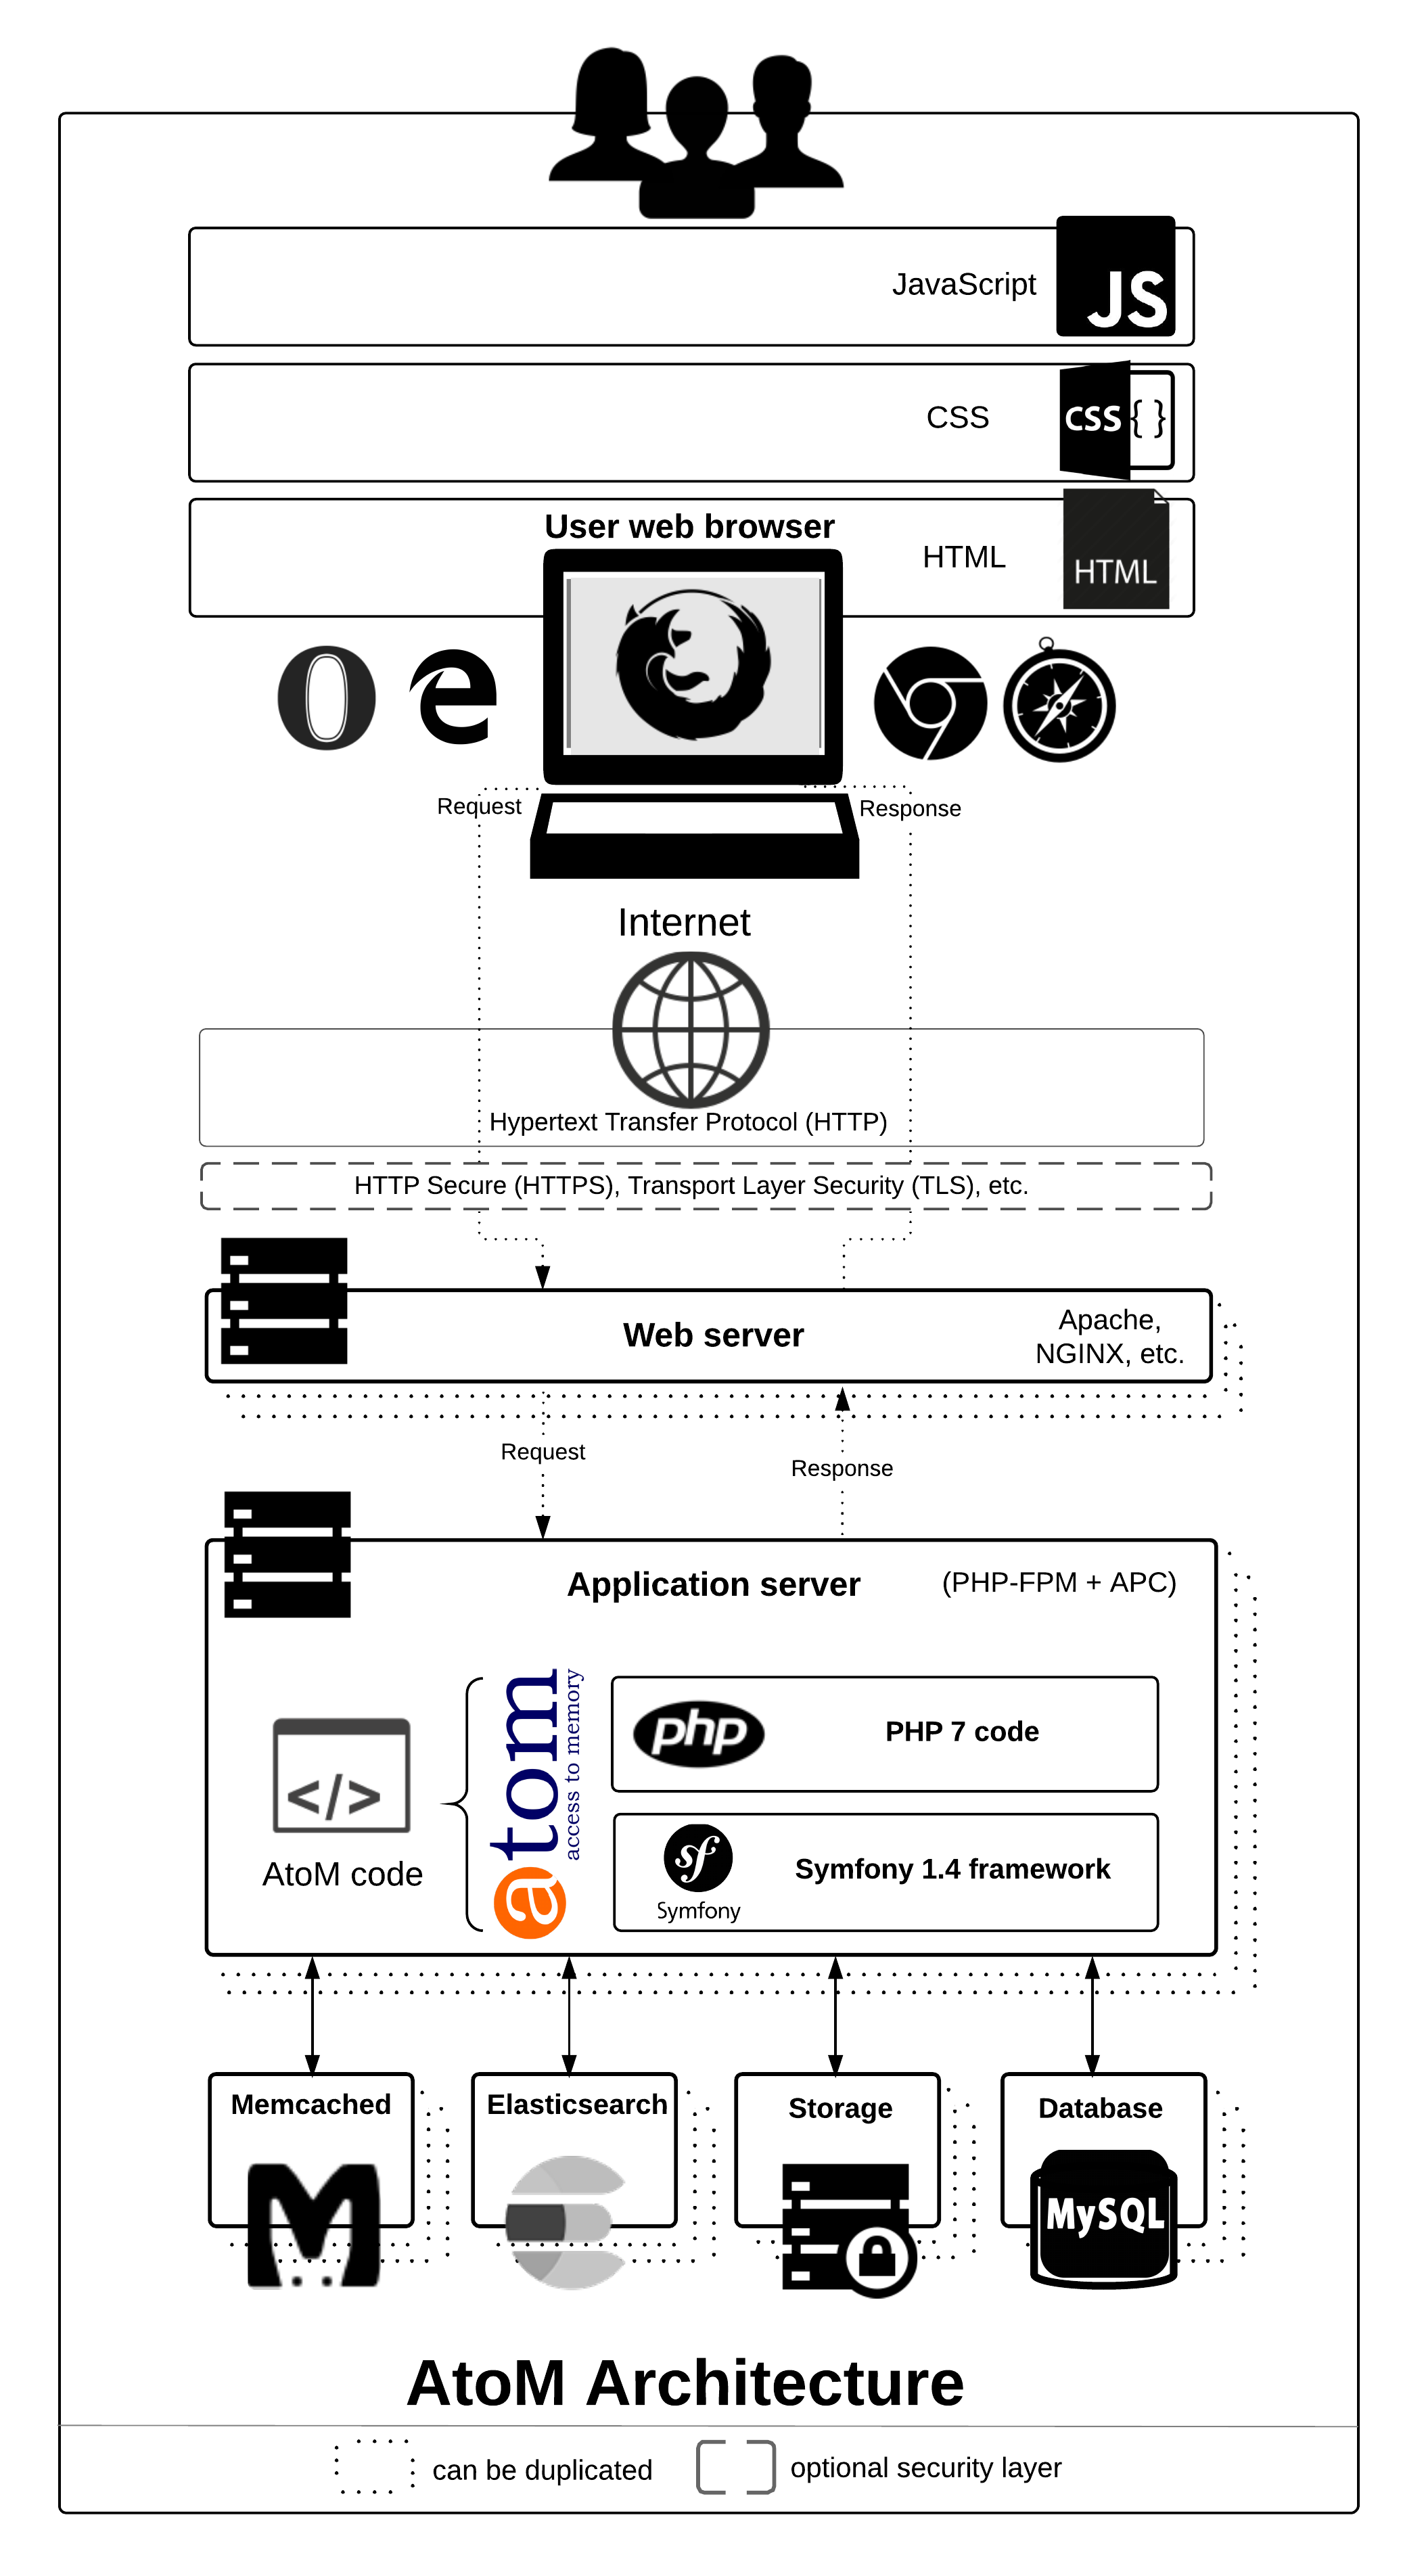
\includegraphics[max width=0.65\textwidth]{Images/what-is-atom.png}
	\end{center}  
	\begin{center}
	Рис 1. Архітектура \textbf{AtoM}.
	\end{center}
	
	\newpage
	
\textbf{AtoM складається з:} 
	
\begin{itemize}
  \item \textbf{HTML-сторінкок}, які надаються браузеру з веб-сервера. Основні два сервера, які використовуються та були протестовані розробниками є \textbf{Nginx} та \textbf{Apache}. 
  \item \textbf{Бази даних}. \textbf{MySQL (8.0)} використовується в розробці, але AtoM використовує рівень абстракції бази даних і тому потенційно сумісний з \textbf{Postgres}, \textbf{SQLite}, \textbf{SQLServer}, \textbf{Oracle}.
  
  \item \textbf{PHP-клієнт}, який керує запитами та відповідями між веб-клієнтами, логікою програми та вмістом програми, що зберігається в базі даних.
  
	\item \textbf{Symphony-Framework}, який організовує складові частини за допомогою об’єктної орієнтації та передових практик веб-дизайну.
	
	\item \textbf{Elasticsearch}. Розподілений пошуковий сервер на базі Apache Lucene, який діє як пошукова та аналітична система програми. Elasticsearch не інтегровано безпосередньо в код AtoM як бібліотеку, а як службу, розгорнуту в тій самій мережі, з якою AtoM взаємодіє через повний API REST.

\end{itemize}	

\end{large}


\section{Технічні вимоги}
Наступна інформація призначена для надання вихідної точки для налаштування вашої системи. Вона надає специфікації для розгортання «все-в-одному», зі всіма службами (тобто nginx, Percona server, ES, memcached), встановленими в одній машині.
\begin{large}

\subsection{Мінімальні вимоги}
\begin{itemize}
    \item Процесор: 2 vCPU @ 2.3 ГГц
    \item Оперативна пам'ять: 7 ГБ
    \item Місце на диску (приблизно): мінімум 50 ГБ для базової частини AtoM, додатковий простір необхідний для підтримки значної кількості цифрових об'єктів.
\end{itemize}

\subsection{Рекомендовані вимоги}
\begin{itemize}
    \item Процесор: 4 vCPU @ 2.3 ГГц
    \item Оперативна пам'ять: 16 ГБ
    \item Місце на диску (приблизно): мінімум 50 ГБ для базової частини AtoM, додатковий простір необхідний для підтримки значної кількості цифрових об'єктів.
\end{itemize}

\subsection{Обов’язкові залежності програмного забезпечення }
\begin{itemize}
    \item Веб-сервер, як-от Apache або Nginx; Artefactual.
    \item Elasticsearch версії 5.x. Elasticsearch 6.0 або новіша версія не підтримується, оскільки вони припинили підтримку деяких API, які все ще використовуються в AtoM.
    \item Java 8 (потрібна для Elasticsearch)
    \item MySQL 8.0
    \item PHP 7.4
    \item Сервер задач Gearman
\end{itemize}
Наступні PHP розширення є обов'язковими:

\begin{itemize}
    \item cURL
    \item JSON
    \item APC (також потрібен apcu-bc)
    \item PDO і PDO-MySQL
    \item XSL
\end{itemize}


\subsection{Інші залежності програмного забезпечення }

\textbf{ImageMagick} — це програмний пакет для створення, редагування, компонування або перетворення растрових зображень. Він може читати та записувати зображення в різних форматах (понад 100), включаючи DPX, EXR, GIF, JPEG, JPEG-2000, PDF, PhotoCD, PNG, Postscript, SVG і TIFF.

\textbf{ImageMagick} використовується в AtoM для створення деривативів зображень (референсного та мініатюри) з головного цифрового об’єкта, включаючи створення деривативів з багатосторінкових TIFF. ImageMagick і Ghostscript потрібні для створення одно- та багатосторінкових PDF деривативів зображень.

\textbf{Ghostscript} — це пакет програмного забезпечення на основі інтерпретатора для мов опису сторінок PostScript компанії Adobe Systems та Portable Document Format (PDF). Основними його цілями є растризація або відтворення таких мов опису сторінок для відображення або друку документів та перетворення між файлами PostScript і PDF.

\textbf{Ghostscript} використовується в AtoM разом із ImageMagick для створення одно- та багатосторінкових PDF деривативів зображень.

\textbf{FFmpeg} — це повне, кросплатформне рішення для запису, конвертування та трансляції аудіо та відео. Він включає libavcodec — провідну бібліотеку аудіо/відео кодеків.

\textbf{FFmpeg} використовується в AtoM для створення відео деривативів, включаючи створення Flash відео деривативу для перегляду у браузері.

\textbf{pdftotext} — це утиліта командного рядка з відкритим кодом для перетворення PDF файлів у звичайні текстові файли, тобто витяг даних з файлів у форматі PDF. Вона безкоштовно доступна та включена за замовчуванням у багатьох дистрибутивах Linux, а також доступна для Windows як частина Xpdf.

\textbf{Apache FOP} (Formatting Objects Processor) — це програма форматування для друку, керована об’єктами форматування XSL (XSL-FO) та незалежний від формату виведення формувач. Це програма на Java, яка зчитує дерево об'єктів форматування (FO) і відображає результат на заданий вихід.

\textbf{Apache FOP} використовується в AtoM для створення PDF-довідників.
\end{large}
\newpage
\section{Встановлення системи AtoM}
\begin{large}

\subsection{Linux}

\subsubsection{Встановлення залежностей}
AtoM 2.8 вимагає MySQL версії 8.0 або вище, оскільки він використовує вирази загальних таблиць.
\begin{lstlisting}[language=bash]
sudo apt update
sudo apt install mysql-server
\end{lstlisting}

\textbf{Порада} \\
Стандартна установка MySQL не є повністю захищеною, але вона містить скрипт безпеки, який можна виконати для покращення налаштувань за замовчуванням:

\begin{lstlisting}[language=bash]
sudo mysql_secure_installation
\end{lstlisting}

При виконанні безпечної інсталяції можна налаштувати обовя'зкову складність паролів.


Нарешті, налаштуємо режими роботи MySQL. Сервер MySQL може працювати в різних SQL-режимах, що впливає на синтаксис SQL, який підтримує MySQL, і на перевірку даних, яку він виконує.


Вставте наступні значення в новий файл за адресою \texttt{/etc/mysql/conf.d/mysqld.cnf} і збережіть:

\begin{lstlisting}
[mysqld]
sql_mode=ERROR_FOR_DIVISION_BY_ZERO,NO_ENGINE_SUBSTITUTION
optimizer_switch='block_nested_loop=off'
\end{lstlisting}

Можна використати редактор nano

\begin{lstlisting}[language=bash]
sudo nano /etc/mysql/conf.d/mysqld.cnf
\end{lstlisting}

Для збереження у nano натисніть Ctr+X і оберіть опцію Yes, після чого нажміть Enter.

Тепер перезапустимо MySQL:

\begin{lstlisting}[language=bash]
sudo systemctl restart mysql
\end{lstlisting}

Встановлюємо сервер для пошуку - Elasticsearch

Сервер пошуку на основі Apache Lucene, розроблений на Java, який забезпечує AtoM численними додатковими функціями, продуктивністю та масштабованістю. Це, ймовірно, найбільша зміна, введена в AtoM 2.x, і ми задоволені результатами.

Ubuntu не надає пакета, але ви можете завантажити його безпосередньо з \textbf{сайту Elasticsearch}, якщо у вас виникають проблеми зі встановленням описаним далі способом.

Переконайтеся, що встановлено Java. У цьому прикладі ми будемо використовувати OpenJDK, але також підійде Oracle JVM.

\begin{lstlisting}[language=bash]
sudo apt install openjdk-11-jre-headless apt-transport-https software-properties-common
\end{lstlisting}

Після успішної установки Java продовжуйте встановлення Elasticsearch. Завантажте та встановіть відкритий ключ підпису, який використовується в їхньому репозиторії:

\begin{lstlisting}[language=bash]
wget -qO - https://artifacts.elastic.co/GPG-KEY-elasticsearch | sudo apt-key add -
\end{lstlisting}

\textbf{Важливо} \\
Не пропустіть тире (\texttt{-}) в кінці цієї команди!

Тепер додайте їхній репозиторій:

\begin{lstlisting}[language=bash]
echo "deb https://artifacts.elastic.co/packages/5.x/apt stable main" | sudo tee -a /etc/apt/sources.list.d/elastic-5.x.list
\end{lstlisting}

Готові до встановлення. Виконайте:

\begin{lstlisting}[language=bash]
sudo apt update
sudo apt install elasticsearch
\end{lstlisting}

Запустіть сервіс та налаштуйте його на автозапуск при завантаженні системи:

\begin{lstlisting}[language=bash]
sudo systemctl enable elasticsearch
sudo systemctl start elasticsearch
\end{lstlisting}

Встановлюємо PHP та German-job-server

Ubuntu 20.04 постачається з PHP 7.4, який значно швидший за попередні версії. Наступна команда встановить PHP разом із рештою PHP-розширень, \textbf{необхідних для AtoM}:


\begin{lstlisting}
sudo apt install php-common php7.4-common php7.4-cli php7.4-curl php7.4-json php7.4-ldap php7.4-mysql php7.4-opcache php7.4-readline php7.4-xml php7.4-mbstring php7.4-xsl php7.4-zip php-apcu php-apcu-bc
\end{lstlisting}

Якщо ви використовуєте Memcached як кешуючий механізм, вам також потрібно встановити php-memcache:

\begin{lstlisting}
sudo apt install php-memcache
\end{lstlisting}

Сервер завдань Gearman необхідний для AtoM, починаючи з версії 2.2.

\begin{lstlisting}
sudo apt install gearman-job-server
\end{lstlisting}


\subsubsection{Завантаження AtoM}
Після встановлення всіх залежностей ми готові завантажити та встановити AtoM. Найбезпечніший спосіб — це завантажити AtoM у вигляді архіву (tarball). Досвідчені користувачі можуть скористатися публічним репозиторієм для завантаження коду.

Всі наступні інструкції припускають, що ми встановлюємо AtoM у каталозі \texttt{/usr/share/nginx} та використовуємо AtoM версії 2.8.0.

\begin{lstlisting}
wget https://storage.accesstomemory.org/releases/atom-2.8.0.tar.gz
sudo mkdir /usr/share/nginx/atom
sudo tar xzf atom-2.8.0.tar.gz -C /usr/share/nginx/atom --strip 1
\end{lstlisting}

\textbf{Примітка:} Архів може бути недоступний, якщо версія ще в розробці. В такому випадку скористайтеся альтернативним методом завантаження, описаним нижче.

Встановіть \texttt{git}:

\begin{lstlisting}
sudo apt install git
\end{lstlisting}

Завантажте код AtoM з гілки stable/2.8.x:

\begin{lstlisting}
sudo mkdir -p /usr/share/nginx/atom
sudo git clone -b stable/2.8.x http://github.com/artefactual/atom.git /usr/share/nginx/atom
\end{lstlisting}

Якщо вам потрібно завантажити лише певну кількість ревізій, скористайтеся командою:

\begin{lstlisting}
git clone -b stable/2.8.x --depth 1 http://github.com/artefactual/atom.git /usr/share/nginx/atom
\end{lstlisting}


Ми використовуємо \textbf{Composer} для встановлення та управління сторонніми бібліотеками PHP. Для встановлення Composer виконайте інструкції на \texttt{https://getcomposer.org/download/}. Після встановлення Composer виконайте команду для встановлення бібліотек:

\begin{lstlisting}
cd /usr/share/nginx/atom
sudo ~/composer.phar install --no-dev
\end{lstlisting}

Або, якщо Composer встановлений глобально:

\begin{lstlisting}
sudo composer install --no-dev
\end{lstlisting}

Для розробницького середовища, де потрібні dev-бібліотеки, використовуйте:

\begin{lstlisting}
sudo ~/composer.phar install
\end{lstlisting}


Після завантаження коду необхідно скомпілювати файли теми.


\begin{lstlisting}
sudo npm install
sudo npm run build
\end{lstlisting}


\begin{lstlisting}
sudo apt install npm make
sudo npm install -g "less@<4.0.0" n
sudo n stable
sudo npm install
sudo npm run build
sudo make -C /usr/share/nginx/atom/plugins/arDominionPlugin
sudo make -C /usr/share/nginx/atom/plugins/arArchivesCanadaPlugin
sudo rm -rf node_modules
\end{lstlisting}

\subsubsection{Створення бази даних}
Припускаючи, що ви використовуєте MySQL на \texttt{localhost}, створіть базу даних за допомогою наступної команди, використовуючи пароль, який ви створили раніше:

\begin{lstlisting}
sudo mysql -h localhost -u root -p -e "CREATE DATABASE atom CHARACTER SET utf8mb4 COLLATE utf8mb4_0900_ai_ci;"
\end{lstlisting}

\textbf{Примітка:} Якщо ви не вказуєте пароль MySQL root після параметра \texttt{-p}, вас буде запрошено ввести його після запуску команди. Якщо ви вказуєте пароль, не залишайте пробіл після \texttt{-p}; наприклад, \texttt{-pPASSWORD}. Пам'ятайте, що введення пароля в командному рядку менш безпечне, оскільки він може бути видимим для інших у файлі \texttt{.bash\_history}.

Зауважте, що база даних названа \texttt{atom}. Ви можете змінити її назву за потреби.

Якщо сервер MySQL не знаходиться на тому ж сервері, що й ваш веб-сервер, замініть \texttt{localhost} на адресу вашого сервера MySQL.

\textbf{Попередження:} Переконайтеся, що ви використовуєте порожню базу даних! Не використовуйте стару базу даних, якщо вона не порожня. Ви завжди можете видалити її за допомогою команди \texttt{DROP DATABASE} і створити знову.


Також рекомендується створити окремого користувача MySQL для AtoM для підвищення безпеки. Нижче наведені команди для створення користувача з іменем \texttt{atom} з паролем \texttt{12345} та призначення йому необхідних прав доступу:

\begin{lstlisting}
sudo mysql -h localhost -u root -p -e "CREATE USER 'atom'@'localhost' IDENTIFIED BY '12345';"
sudo mysql -h localhost -u root -p -e "GRANT ALL PRIVILEGES ON atom.* TO 'atom'@'localhost';"
\end{lstlisting}

\textbf{Примітка:} Права \texttt{INDEX}, \texttt{CREATE} та \texttt{ALTER} необхідні під час процесу встановлення або оновлення AtoM. Вони можуть бути видалені з користувача після завершення установки, або ви можете обмежити права користувача в файлі \texttt{config.php}.
\subsubsection{Інсталювання}

Тепер ви готові запустити інсталятор. Це проста команда, яка налаштовує AtoM відповідно до вашого середовища, додає необхідні таблиці та початкові дані до бази даних і створює індекс Elasticsearch.

\begin{lstlisting}
cd /usr/share/nginx/atom
php symfony tools:install
\end{lstlisting}

Інсталятор запитає деталі конфігурації, такі як місцезнаходження сервера бази даних, ім’я користувача, пароль тощо. Приклад конфігурації:

\begin{itemize}
    \item Database host: \texttt{localhost}
    \item Database port: \texttt{3306}
    \item Database name: \texttt{atom}
    \item Database user: \texttt{atom}
    \item Database password: \texttt{12345}
    \item Search host: \texttt{localhost}
    \item Search port: \texttt{9200}
    \item Search index: \texttt{atom}
\end{itemize}

Надайте права на каталог AtoM:

\begin{lstlisting}
sudo chown -R www-data:www-data /usr/share/nginx/atom
sudo chmod -R 755 /usr/share/nginx/atom
\end{lstlisting}

\textbf{Налаштування Worker для Gearman}

Gearman використовується для підтримки асинхронних завдань. Створіть файл сервісу:

\begin{lstlisting}
sudo nano /usr/lib/systemd/system/atom-worker.service
\end{lstlisting}

Вставте наступне:

\begin{lstlisting}
[Unit]
Description=AtoM worker
After=network.target

[Service]
Type=simple
User=www-data
Group=www-data
WorkingDirectory=/usr/share/nginx/atom
ExecStart=/usr/bin/php7.4 -d memory_limit=-1 -d error_reporting="E_ALL" symfony jobs:worker
Restart=on-failure
RestartSec=30

[Install]
WantedBy=multi-user.target
\end{lstlisting}

Перезавантажте, активуйте і запустіть worker:

\begin{lstlisting}
sudo systemctl daemon-reload
sudo systemctl enable atom-worker
sudo systemctl start atom-worker
\end{lstlisting}

\textbf{Налаштування PHP-FPM для AtoM}

Встановіть PHP-FPM та додайте конфігураційний пул:

\begin{lstlisting}
sudo apt install php7.4-fpm
sudo nano /etc/php/7.4/fpm/pool.d/atom.conf
\end{lstlisting}

Вставте наступне налаштування:

\begin{lstlisting}
[atom]
user = www-data
group = www-data
listen = /run/php/php7.4-fpm.atom.sock
listen.owner = www-data
listen.group = www-data
listen.mode = 0600
pm = dynamic
pm.max_children = 30
pm.start_servers = 10
pm.min_spare_servers = 10
pm.max_spare_servers = 10
pm.max_requests = 200
\end{lstlisting}

Перезапустіть PHP-FPM:

\begin{lstlisting}
sudo systemctl enable php7.4-fpm
sudo systemctl start php7.4-fpm
\end{lstlisting}

\textbf{Налаштування Nginx для AtoM}

Встановіть Nginx і створіть конфігурацію для AtoM:

\begin{lstlisting}
sudo apt install nginx
sudo nano /etc/nginx/sites-available/atom
\end{lstlisting}

Додайте наступне налаштування:

\begin{lstlisting}
server {
    listen 80;
    server_name localhost;

    root /usr/share/nginx/atom;
    index index.php;

    location / {
        try_files $uri $uri/ /index.php?$query_string;
    }

    location ~ \.php$ {
        include snippets/fastcgi-php.conf;
        fastcgi_pass unix:/run/php/php7.4-fpm.atom.sock;
    }

    location ~ /\.ht {
        deny all;
    }
}
\end{lstlisting}

Активуйте конфігурацію та перезапустіть Nginx:

\begin{lstlisting}
sudo ln -s /etc/nginx/sites-available/atom /etc/nginx/sites-enabled/
sudo systemctl restart nginx
\end{lstlisting}


Тепер відкрийте браузер і перейдіть за адресою \texttt{http://localhost}, щоб перевірити, чи працює AtoM.

\subsection{Windows}
Кожен елемент програмного забезпечення, \textbf{необхідний для AtoM}, сумісний з Windows. Однак слід знати, що процес може бути зовсім не простим, якщо ви не знайомі з серверними середовищами під платформою Windows.
\end{large}


\section{Конфігурація}
\begin{large}
Система \textbf{AtoM} надає багато можливостей щодо конфігурації. У цьому розділі буде описано як модерацію системи зі сторони web-сторінки, використовуючи роль адміністратора, так і ручну зміну налаштувань у внутрішніх файлам самого проекту.

\subsection{Маніпуляція налаштуваннями з веб-сторінки}

\subsection{Конфігураційні файли}

\end{large}

\section{Постскриптум}
Маємо дякувати за прочитання

\end{document}
